\documentclass{article}

\usepackage{tikz}

\usetikzlibrary{arrows.meta}
\usetikzlibrary{calc}


\title{Vectors with LaTeX Part 2: Diagrams}
\author{Chris Webb, LaTeX Snippets}

\colorlet{gridlines}{gray!25}
\colorlet{axes}{gray}


\begin{document}

\maketitle


\section{An Empty Grid}

\begin{center}
    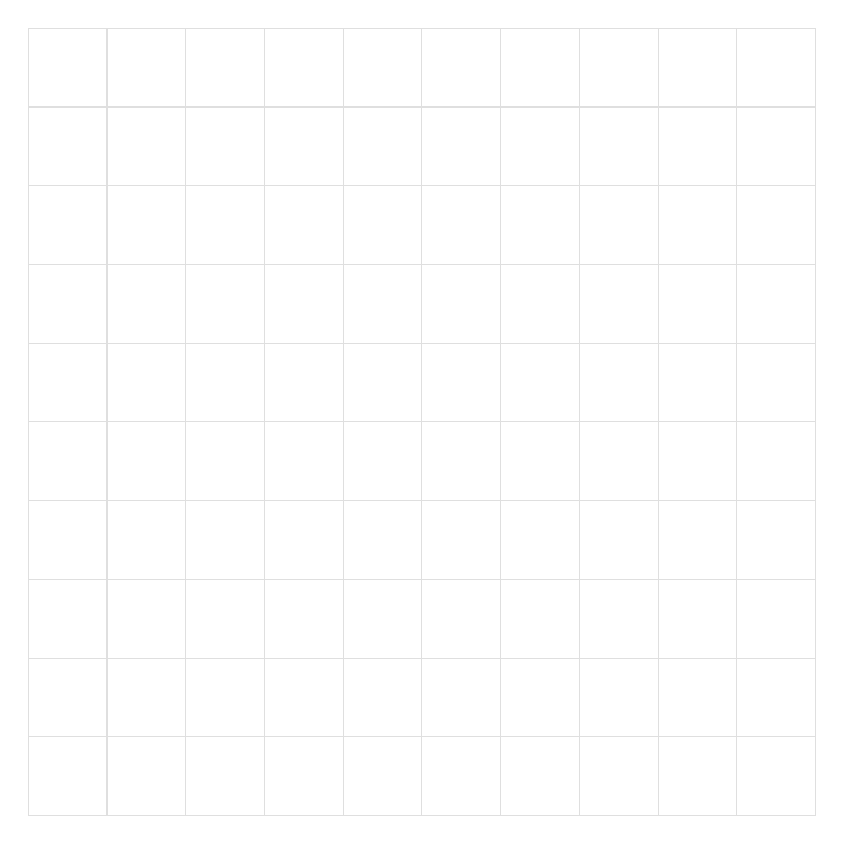
\begin{tikzpicture}
        \draw(0,0)[gridlines] grid(10,10);
    \end{tikzpicture}
\end{center}


\section{Adding Axis Values}

\begin{center}
    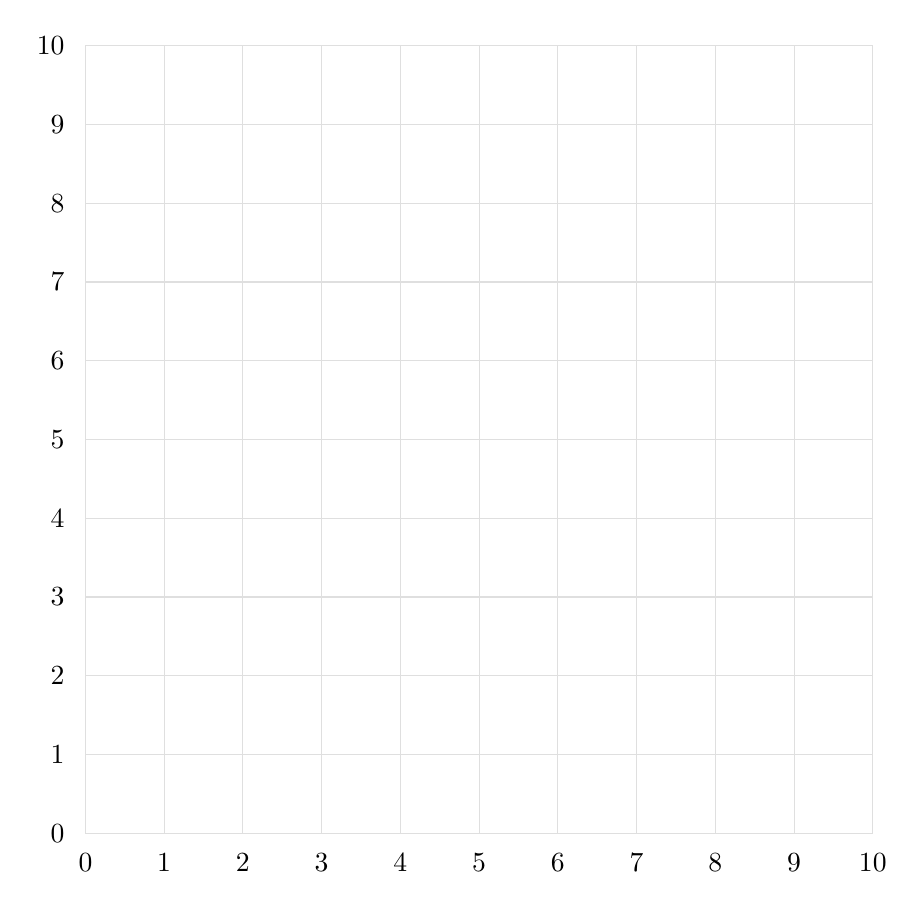
\begin{tikzpicture}
        \draw(0,0)[gridlines] grid(10,10);
        \foreach \x in {0,...,10}
        {
            \node[anchor=north, yshift=-4pt] at (\x,0) {\x};
        }
        \foreach \y in {0,...,10}
        {
            \node[anchor=east, xshift=-4pt] at (0,\y) {\y};
        }
    \end{tikzpicture}
\end{center}


\section{Adding Vector Lines with Arrows}

\begin{center}
    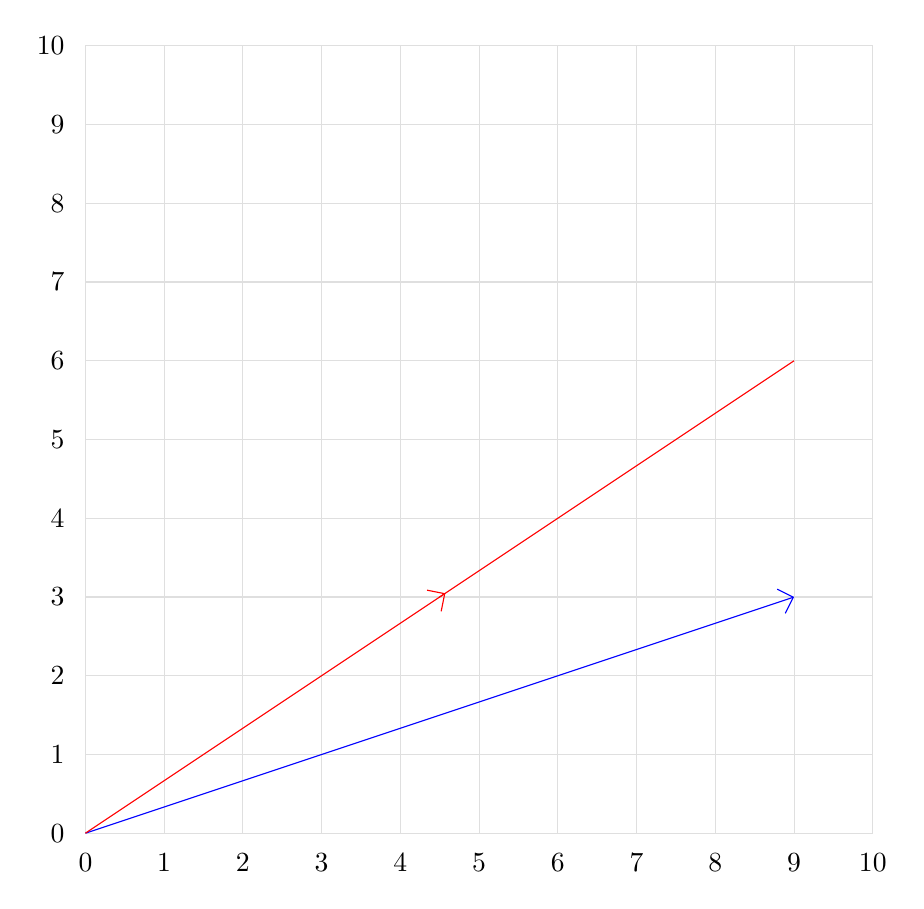
\begin{tikzpicture}
        % vector coordinates
        \coordinate (A) at (0,0);
        \coordinate (B) at (9,3);
        \coordinate (C) at (9,6);
        % grid
        \draw(0,0)[gridlines] grid(10,10);
        \foreach \x in {0,...,10}
        {
            \node[anchor=north, yshift=-4pt] at (\x,0) {\x};
        }
        \foreach \y in {0,...,10}
        {
            \node[anchor=east, xshift=-4pt] at (0,\y) {\y};
        }
        % vector: arrow at end 
        \draw[-{Straight Barb[scale=2]}][blue] (A) -- (B);
        % vector: arrow in middle 
        \draw (A)[red] -- (C) node [midway, sloped, allow upside down] 
        {$\tikz \draw[-{Straight Barb[scale=2]}] (0,0) -- (0.1,0);$};
    \end{tikzpicture}
\end{center}


\section{Adding Start and End Point Letters}

\begin{center}
    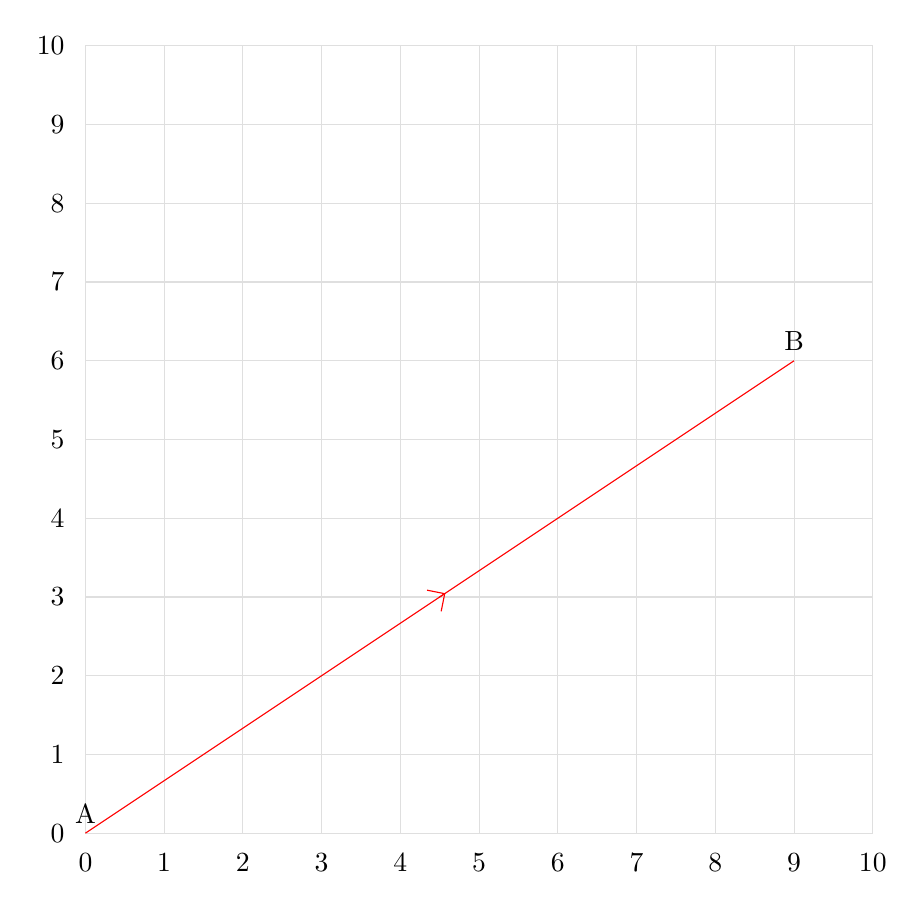
\begin{tikzpicture}
        \coordinate (A) at (0,0);
        \coordinate (B) at (9,6);
        % grid
        \draw(0,0)[gridlines] grid(10,10);
        \foreach \x in {0,...,10}
        {
            \node[anchor=north, yshift=-4pt] at (\x,0) {\x};
        }
        \foreach \y in {0,...,10}
        {
            \node[anchor=east, xshift=-4pt] at (0,\y) {\y};
        }
        % ~~~~~~~~~~~~~~~~~
        \draw (A)[red] -- (B) node [midway, sloped, allow upside down] 
        {$\tikz \draw[-{Straight Barb[scale=2]}] (0,0) -- (0.1,0);$};
        \node[anchor=south] at (A) {A};
        \node[anchor=south] at (B) {B};
    \end{tikzpicture}
\end{center}


\section{Adding a Name}

\begin{center}
    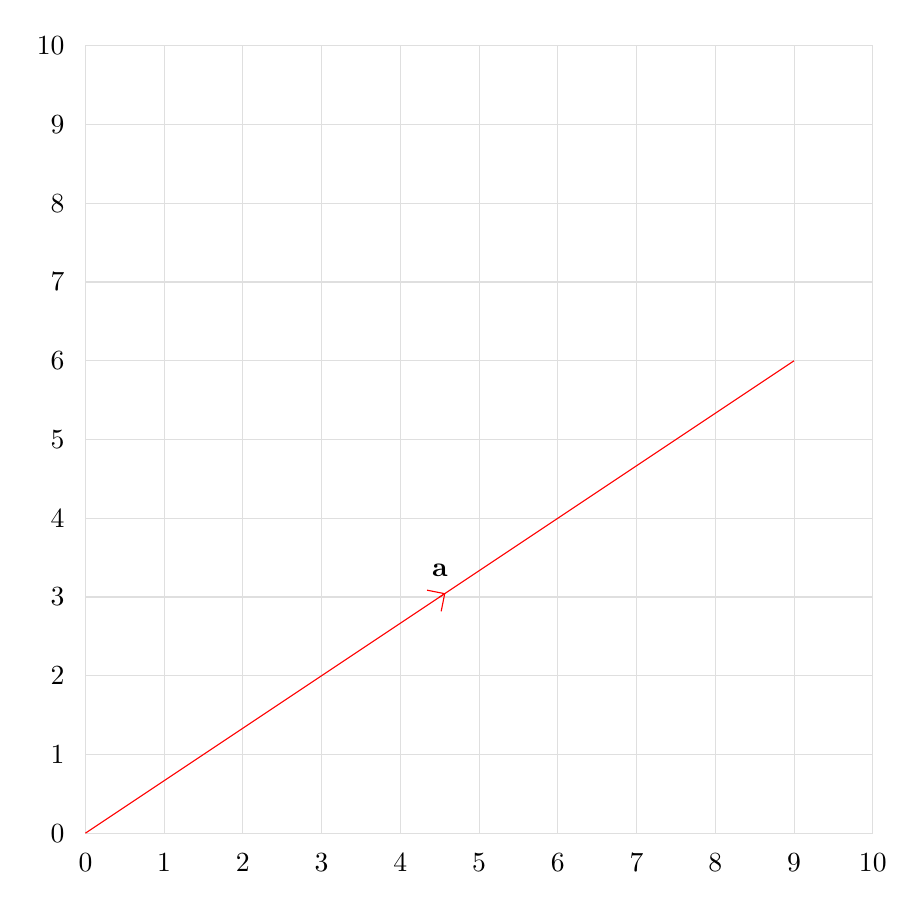
\begin{tikzpicture}
        % start and end points
        \coordinate (A) at (0,0);
        \coordinate (B) at (9,6);
        % name position at midpoint shifted up by 4pt
        \coordinate (name) at ($(A)!0.5!(B)+(0pt,4pt)$);
        % grid
        \draw(0,0)[gridlines] grid(10,10);
        \foreach \x in {0,...,10}
        {
            \node[anchor=north, yshift=-4pt] at (\x,0) {\x};
        }
        \foreach \y in {0,...,10}
        {
            \node[anchor=east, xshift=-4pt] at (0,\y) {\y};
        }
        % vector line
        \draw (A)[red] -- (B) node [midway, sloped, allow upside down] 
        {$\tikz \draw[-{Straight Barb[scale=2]}] (0,0) -- (0.1,0);$};
        % name letter
        \node[anchor=south] at (name) {$\mathbf{a}$};
    \end{tikzpicture}
\end{center}


\section{Alternative Arrows}

\begin{center}
    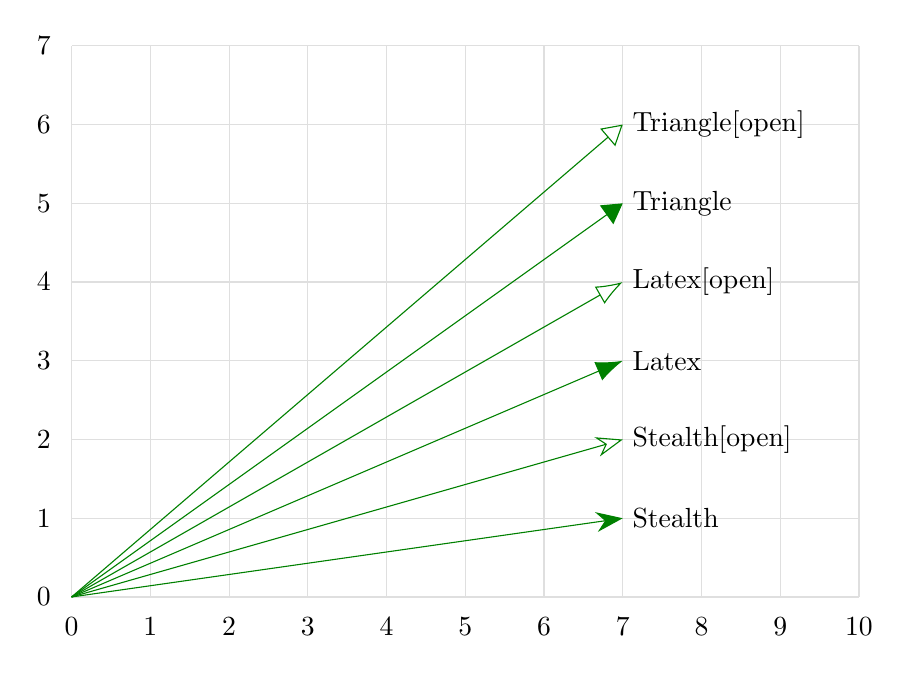
\begin{tikzpicture}
        % coordinates
        \coordinate (A) at (0,0);
        % grid
        \draw(0,0)[gridlines] grid(10,7);
        \foreach \x in {0,...,10}
        {
            \node[anchor=north, yshift=-4pt] at (\x,0) {\x};
        }
        \foreach \y in {0,...,7}
        {
            \node[anchor=east, xshift=-4pt] at (0,\y) {\y};
        }
        % arrows
        \draw[-{Stealth[scale=2]}][green!50!black] (A) -- 
        (7,1) node[right][black] {Stealth};
        \draw[-{Stealth[open, scale=2]}][green!50!black] (A) -- 
        (7,2) node[right][black] {Stealth[open]};
        \draw[-{Latex[scale=2]}][green!50!black] (A) -- 
        (7,3) node[right][black] {Latex};
        \draw[-{Latex[open, scale=2]}][green!50!black] (A) -- 
        (7,4) node[right][black] {Latex[open]};
        \draw[-{Triangle[scale=2]}][green!50!black] (A) -- 
        (7,5) node[right][black] {Triangle};
        \draw[-{Triangle[open, scale=2]}][green!50!black] (A) -- 
        (7,6) node[right][black] {Triangle[open]};
    \end{tikzpicture}
\end{center}


\section{Another Empty Grid}

\begin{center}
    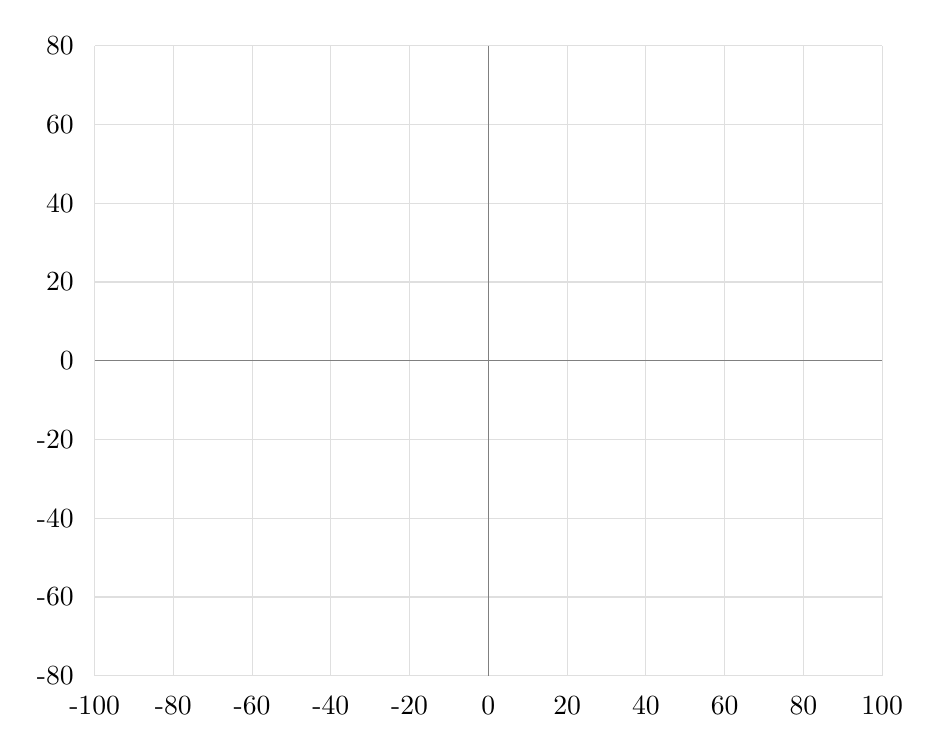
\begin{tikzpicture}[scale=0.05]
        \draw[step=20] (-100,-80)[gridlines] grid(100,80);
        \draw[axes](-100,0)--(100,0);
        \draw[axes](0,80)--(0,-80);
        \foreach \x in {-100,-80,...,100}
        {
            \node[scale=1.0, anchor=north, yshift=-4pt] at (\x,-80) {\x};
        }
        \foreach \y in {-80,-60,...,80}
        {
            \node[scale=1.0, anchor=east, xshift=-4pt] at (-100,\y) {\y};
        }
    \end{tikzpicture}
\end{center}


\end{document}